\section{\content{電腦中的漢字}{电脑中的汉字}}\label{section:chinese characters on computers}
\content{進入現代以後,電腦成為了人們讀寫漢字的新媒介。如今資訊科技高度發達,許多人使用電腦來讀寫的時間已經遠遠超過了使用紙筆。媒介的改變當然會帶來讀寫方式的改變,於是人們設計數位字型以供顯示漢字,設計輸入法以供鍵入漢字。}{进入现代以后,电脑成为了人们读写汉字的新媒介。如今信息技术高度发达,许多人使用电脑来读写的时间已经远远超过了使用纸笔。媒介的改变当然会带来读写方式的改变,于是人们设计数码字型以供显示汉字,设计输入法以供键入汉字。}\par
\content{在本節,筆者將簡要介紹一些電腦漢字相關的知識。如果你對「亂碼」的來歷感到好奇,對中文輸入法的選擇有些困惑,或者是想了解印刷體與手寫體的區別,那就一定不要錯過本節的內容。}{在本节,笔者将简要介绍一些电脑汉字相关的知识。如果你对“乱码”的来历感到好奇,对中文输入法的选择有些困惑,或是是想了解印刷体与手写体的区别,那就一定不要错过本节的内容。}\par
\subsection{\content{中文輸入法}{中文输入法}}
\content{我們一般所說的「輸入法」可以分解成兩個層次的概念:\textbf{輸入法方案}與\textbf{輸入法程式}。很多人在比較輸入法時,經常把方案之間的比較與程式之間的比較相混淆,從而引起很多不必要的爭執。筆者認為自己有義務對這些概念加以解釋。}{我们一般所说的“输入法”可以分解成两个层次的概念:\textbf{输入法方案}与\textbf{输入法程序}。很多人在比较输入法时,经常把方案之间的比较与程式之间的比较相混淆,从而引起很多不必要的争执。笔者认为自己有义务对这些概念加以解释。}\par
\subsubsection{\content{輪入法方案}{输入法方案}}
\content{輸入法方案關乎於每個字的編碼。在倉頡碼中「輸」的編碼是「十十人一弓」,對應到鍵盤上就是「jjomn」;在漢語全拼中的編碼則是「shu」,對應鍵盤上的「shu」。}{输入法方案关乎于每个字的编码。在仓颉码中“输”的编码是「大手人一弓」,对应到键盘上就是“kqomn”;在汉语全拼中的编码则是“shu”,对应键盘上的“shu”。}\par
\content{一種最死板的輸入法方案是,直接把所有漢字亂序編碼。我們只要強記這些編碼,就可以在鍵盤上打出任何一個我們想要的字。Unicode輸入法便是如此,我們只需敲下「輸」的編碼「8f38」就可以得到這個字。}{一种最死板的输入方案是,直接把所有汉字乱序编码。我们只要强记这些编码,就可以在键盘上打出任何一个我们想要的字。Unicode便入法便是如此,我们只需敲下“输”的编码“8f93”就可以得到这个字。}\par
\content{這類編碼的缺陷顯而易見:各個漢字與其編碼之間沒有任何邏輯關聯。為了正常使用,人們必須強行記住每個字的編碼,而這樣巨大的記憶量將使人望而卻步。所以人們當然更傾向於把漢字與其編碼關聯起來,用「推導」代替不必要的「記憶」。這種邏輯關聯的本質就是直接分析一個字的音、形、義,由此推算出編碼。分析字義並不可行,所以主流的中文輸入法要麼是基於字音的\textbf{音碼輸入法},要麼是基於字形的\textbf{形碼輸入法}。}{这类编码的缺陷显而易见:各个汉字与其编码之间没有任何逻辑关联。为了正常使用,人们必须强行记住每个字的编码,而这样巨大的记忆量将使人望而却步。所以人们当然更倾向于反汉字与其编码关联起来,用“推导”代替不必要的“记忆”。这种逻辑关联的本质就是直接分析一个字的音、形、义,由此推算出编码。分析字义并不可行,所以主流的中文输入法要么是基于字音的\textbf{音码输入法},要么是基于字形的\textbf{形码输入法}。}\par
\content{音碼輸入法的拆字思路比較簡單:根據漢語拼音、注音符號或粵語拼音等,把一個字的讀音轉換成編碼。「輸」的粵語拼音是「syu」,對應到粵拼方案上就是「syu」;拼音是「shu」,對應到自然碼雙拼方案上就是「uu」\footnote{在自然碼雙拼中,聲母「sh」對應到「u」鍵。此方案還提供了字形輔助碼,但那不是必須掌握的部分。};注音是「ㄕㄨ」,對應到大千式注音方案上就是「gj」。對於受過良好拼音/注音教育的人來說,字音輸入法的優點就是上手簡單,易學易用——無論你是否會寫,只要你知道它的讀音,你就知道它在拼音/注音中如何拆,然後你只需要在鍵盤上敲下對應的鍵\footnote{在台灣,許多電腦鍵盤不止印有英數字母,還印有注音符號甚至倉頡、大易字根,所以在鍵盤上就可以直接找到注音符號的位置。}就可以了。}{音码输入法的拆字思路比较简单:根据汉语拼音、注音符号或粵语拼音等,把一个字的读音转换成编码。“输”的粵语拼音是“syu”,对应到粵拼方案上就是“syu”;拼音是“shu”,对应到自然码双拼方案上就是“uu”\footnote{在自然码双拼中,声母“sh”对应到“u”键。此方案还提供了字形辅助码,但那不是必须掌握的部分。};注音是“ㄕㄨ”,对应到大千式注音方案上就是“gj”。对于受过良好拼音/注音教育的人来说,字音输入法的优点就是上手简单,易学易用——无论你是否会写,只要你知道它的读音,你就知道它在拼音/注音中如何拆,然后你只需要在键盘上敲下对应的键\footnote{在台湾,许多电脑键盘不止印有英数字母,还印有注音符号甚至仓颉、大易字根,所以在键盘上就可以直接找到注音符号的位置。}就可以了。}\par
\begin{wrapfigure}{O}{.38\textwidth}
	\centering
	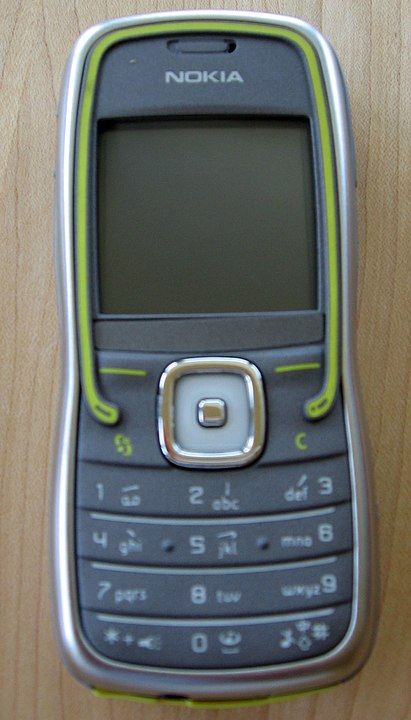
\includegraphics[width=.38\textwidth]{Nokia_5500.jpg}
	\caption{\content{一款諾基亞傳統型手機}{一款諾基亞傳統型手機}}
	\label{figure:一款諾基亞傳統型手機}
	\footnotesize{\color{darkgray}\content{鍵盤1-5對應有筆順鍵}{键盘1-5对应有笔顺键}}
\end{wrapfigure}
\content{音碼輸入法往往都基於既有的拼音/注音方案,在拆字思路上大同小異;但形碼輸入法就五花八門了。最細碎的筆畫輸入法把每個字的筆畫都拆開來,分成「橫竪撇點折」五類,每一筆都是一碼,那麼「輸」字要敲上足足16碼。因為編碼過長,輸入效率很低,所以幾乎沒有人再使用了,只在傳統型手機的九鍵鍵盤中還有保留(\cref*{figure:一款諾基亞傳統型手機})。}{音码输入法往往都基于既有的拼音/注音方案,在拆字思路上大同小异;但形码输入法就五花八门了。最细碎的笔画输入法把每个字的笔画都拆开来,分成“横竖撇点折”五类,每一笔者是一码,那么“输”字要敲上足足13码。因为编码过长,输入效率很低,所以几乎没有人再使用了,只在传统型手机的九键键盘中还有保留(\cref*{figure:一款諾基亞傳統型手機})。}\par
\content{很多字的成分非常複雜,一筆一畫寫出來不現實,所以我們需要限制每個字的編碼長度,只取其中的若干成分,作為\textbf{字根}。一個字的編碼將根據它的字根及結構來確定。四角號碼便是如此。它規定一個字必須編四碼\footnote{這里不考慮附角。如果考慮附角的話,應是五碼。},在編碼時分別看這個字左上角、右上角、左下角、右下角的字根形狀,再把字根轉換為對應的數字。還以「輸」字為例,它的左上角和左下角是連起來的一個「插」畫,所以左上角取「5」,左下角用「0」代替;右上角的「人」是「八」畫,取「8」;右下角的「亅」是「垂」畫,取「2」。所以「輸」字的四角號碼為「5802」。}{很多字的成分非常复杂,一笔一画写出来不现实,所以我们需要限制每个字的编码长度,只取其中的若干成分,作为\textbf{字根}。一个字的编码将根据它的字根及结构来确定。四角号码便是如此。它规定一个字必须编四码\footnote{这里不考虑附角。如果考虑附角的话,应是五码。},在编码时分别看这个字左上角、右上角、左下角、右下角的字根形状,再把字根转换为对应的数字。还以“输”字为例,这个字左上角的“𠂇”是“叉”画,取“4”;右上角的“人”是“八”画,取“8”;左下角的“𰀁”是“插”画,取“5”;右下角的“亅”是“垂”画,取“2”。所以“轮”字的四角号码为“4852”。}\par
\content{四角號碼發明於20世紀初。當時四角號碼並非用於打字,而是用於「檢字」\footnote{最典型的檢字就是根據字形查字典。很多人只會用部首檢字法,即:先根據部首的筆畫數量找到部首所在頁,再根據剩餘的筆畫數量從同部首的字中找到目標字。這種檢字方法容易學,但效率偏低,因為既要確定部首,又要數出筆畫數量,還需要在很多字中找到目標字。用四角號碼來檢字就方便很多。}。後來有人把四角號碼加以改良,製成縱橫輸入法。縱橫碼的思路也是根據漢字四角的成分來取碼。}{四角号码发明于20世世纪初。当时的四角号码并非用于打字,而是用于“检字”\footnote{最典型的检字就是根据字形查字典。很多人只会用部首检字法,即:先根据部首的笔画数量找到部首所在页,再根据剩余的笔画数量从同部首的字中找到目标字。这种检字方法容易学,但效率偏低,因为既要确这部首,又要数出笔画数量,还需要在很多字中找到目标字。用四角号码来检字就方便很多。}。后来有人把四角号码加以改良,制成纵横输入法。纵横码的思路也是根据汉字四角的成分来取码。}\par
\content{筆順、四角和縱橫所需的編碼鍵較少,所以在九鍵鍵盤或電腦小鍵盤上仍有用武之地;但在大鍵盤上,我們完全可以把字根分得更細緻。大易輸入法和行列40輸入法使用了40個鍵;行列30輸入法使用了30個鍵;鄭碼、徐碼、嘸蝦米使用了26個鍵;倉頡輸入法\footnote{不含六代倉頡輸入法(或曰「蒼頡輸入法」)。}、五筆字型輸入法使用了25個鍵\footnote{倉頡的「重」和五筆的「z」都不是必需的,不計入。}。}{笔顺、四角和纵横所需的编码键较少,所在在九键键盘或电脑小键盘上仍有用武之地;但在大键盘上,我们完全可以把字根分得更细致。大易输入法和行列40输入法使用了40个键;行列30输入法使用了30个键;郑码、呒吓米输入法使和了26个键;仓颉输入法\footnote{不含六代仓颉输入法(或曰“苍颉输入法”)。}、五笔字型输入法使用了25个键\footnote{仓颉的“重”和五笔的“z”都不是必需的,不讲入。}。}\par
\content{不同的形碼輸入法可能採用完全不同的字根體系、拆字方式和編碼方式。但無論如何,只要給定一套規則,我們就可以對任何一個字進行編碼。這就是「輸入法方案」所關注的問題。}{不同的形码输入法可能采用完全不同的字根体系,拆字方式和编码方式。但无论如何,只要给定一套规则,我们就可以对任何一个字进行编码。这就是“输入法方案”所关注的问题。}\par
